\chapter{The CMS experiment at the LHC}
\label{sec:cms}

\section{The Large Hadron Collider}

The Large Hadron Collider (LHC)~\cite{lhcjinst}\footnote{Unless otherwise specified, all technical specifications of the LHC are derived from Reference~\cite{lhcjinst}} is a circular particle accelerator, 27 km in circumference and between 40 and 175 m below the surface of the French-Swiss border. 
Designed to collide protons at a maximum center-of-mass energy $\sqrt{s} = 14$ TeV, the LHC has delivered collisions at $\sqrt{s}=7,8$ TeV (Run 1) and $\sqrt{s} = 13$ TeV (Run 2); the target energy $\sqrt{s} = 14$ TeV will be reached in Run 3. 
In addition to protons, the LHC accelerates and collides heavy nuclei (Pb and Xe) at lower values of $\sqrt{s}$. 
In this thesis, we focus exclusively on data recorded from proton collisions during Run 2. 

\begin{figure}[]
    \begin{center}
        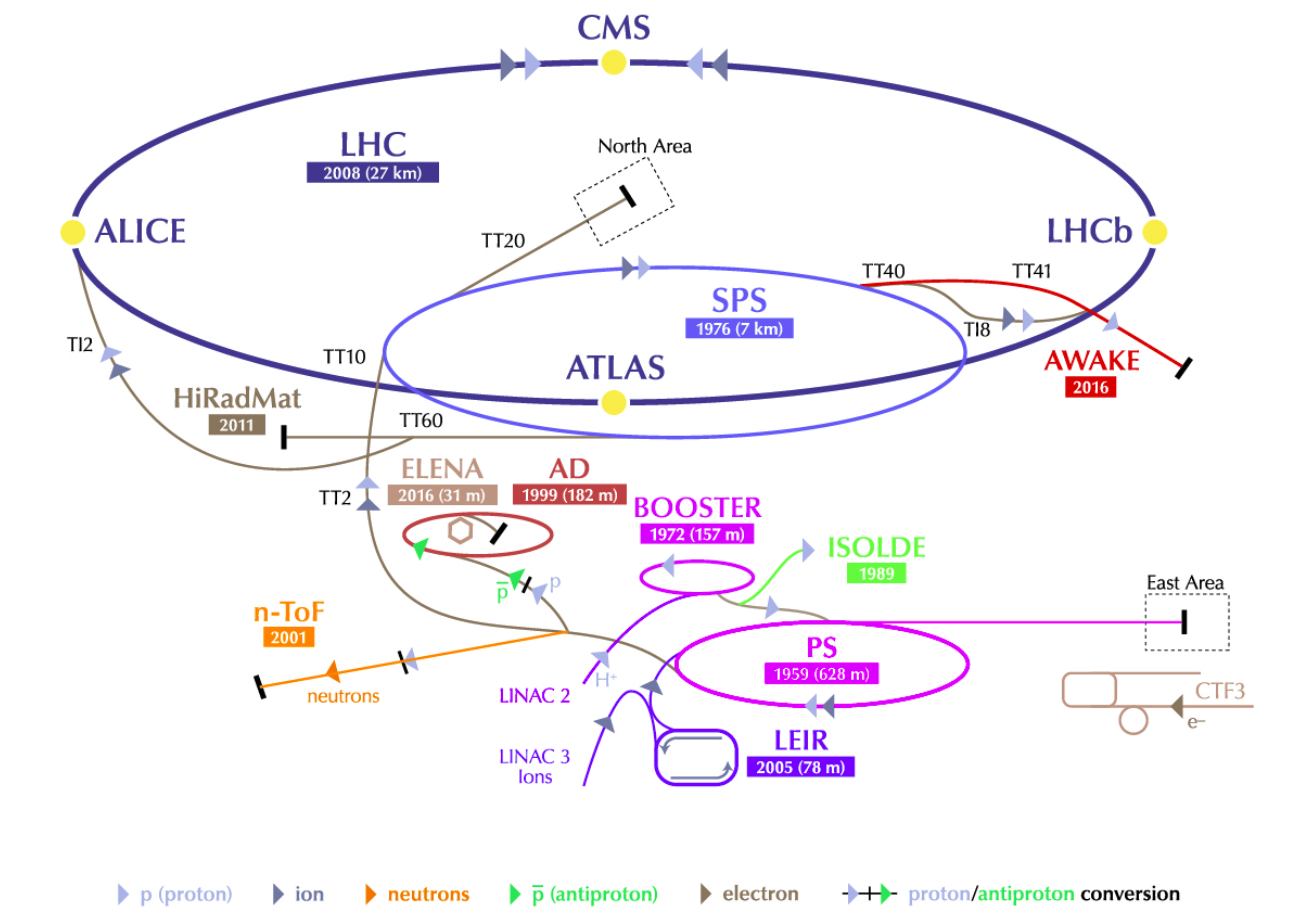
\includegraphics[width=0.8\textwidth]{figures/cms/lhc.png}
        \caption{Diagram of the CERN accelerator complex, adapted from Reference~\cite{lhcpic}. 
                 The LHC (dark blue) is fed protons (and heavy ions) by a chain of intermediate accelerators, beginning with LINAC2 (dark pink).}
        \label{fig:cms:lhc}
    \end{center}
\end{figure}

Protons are brought to the LHC by the multi-stage process~\cite{lhctdr3} depicted in Figure~\ref{fig:cms:lhc}.
Hydrogen atoms are stripped of electrons and accelerated by LINAC2 (a linear accelerator) to a kinetic energy of $50$ MeV.
LINAC2 then feeds the protons into the Booster ring (final energy of $1.4$ GeV), followed by the Proton Synchrotron ($26$ GeV).
From the PS, the protons are injected into the Super Proton Synchrotron ($450$ GeV).
Protons exit the SPS and enter the LHC at one of two places, corresponding to two different beams traveling in opposite directions.
The two beams intersect in eight places along the LHC, four of which are instrumented by a detector experiment: CMS, ATLAS, LHCb, and ALICE. 

Each proton beam in the LHC is accelerated by eight superconducting cavities exerting radio frequency longitudinal (i.e. parallel to beam direction) electric fields with a frequency of $400$ MHz,
The maximum RF voltage seen by each beam is 16 MV per revolution.
The physical and temporal design of the RF system creates bunches of protons (corresponding to nodes of the oscillating field) approximately 7.5 cm in length and separated by 25 ns. 
Superconducting NbTi dipole magnets bend the two proton beams in opposite directions as they travel around the ring. 
Each of the 1232 dipoles is 14 m long and exerts a transverse $B$ field between $0.54$ and $8.33$ T.
To achieve such high $B$ fields, the magnets are cooled to 2 K by superfluid helium.
In addition, a number of quadrupole magnets are used to focus and match the beams between the dipoles\footnote{Full details on the various quadrupoles can be found in Table 3.7 of Reference~\cite{lhcjinst}.}.

In addition to the center-of-mass energy $\sqrt{s}$, the other figure of merit is the number of events producing interesting physics processes, which is defined as:
\begin{equation} 
    N(pp\rightarrow X) = \int dt L \sigma(pp\rightarrow X)
\end{equation}
where $\sigma$ is the cross section of the relevant process and $L$ is the instantaneous luminosity of the LHC. 
The cross section is fixed by nature, and so increasing the luminosity is the only handle to increase $N$. 
The instantaneous luminosity of two Gaussian beams is given by~\cite{lhcjinst}:
\begin{equation}
    L = \frac{N_b^2 n_b f_\mathrm{rev} \gamma F}{4\pi\epsilon \beta^*}
\end{equation}
where:
\begin{itemize}
    \item[$N_b$ $=$] particles per bunch
    \item[$n_b$ $=$] bunches per beam 
    \item[$f_\mathrm{rev}$ $=$] frequency of revolution 
    \item[$\gamma$ $=$] $E/m$ of beam 
    \item[$\epsilon$ $=$] emittance of beam 
    \item[$\beta^*$ $=$] beta function at collision point 
    \item[$F$ $=$] factor accounting for beam intersection geometry
\end{itemize}
The instantaneous luminosity evolves as a function of time, primarily due to $n_b$ and $N_b$ being modified by collisions.
The total integrated luminosity after time $T$ is:
\begin{equation}
    L_\mathrm{int} = \int_0^T dt L(t) = L(0) \tau_L \left(1 - e^{-T/\tau_L}\right)
\end{equation}
where $\tau_L \approx 15$ h is the characteristic beam loss timescale and $L(0)$ is the instantaneous luminosity at $T=0$.
The LHC is designed to deliver $L(0) \sim \mathcal{O}(10^{34})$ cm$^{-2}$s$^{-1}$. 
Figure~\ref{fig:cms:lumi} shows the total luminosity delivered by the LHC and recorded by CMS during the 2016 portion of Run 2. 

\begin{figure}[]
    \begin{center}
        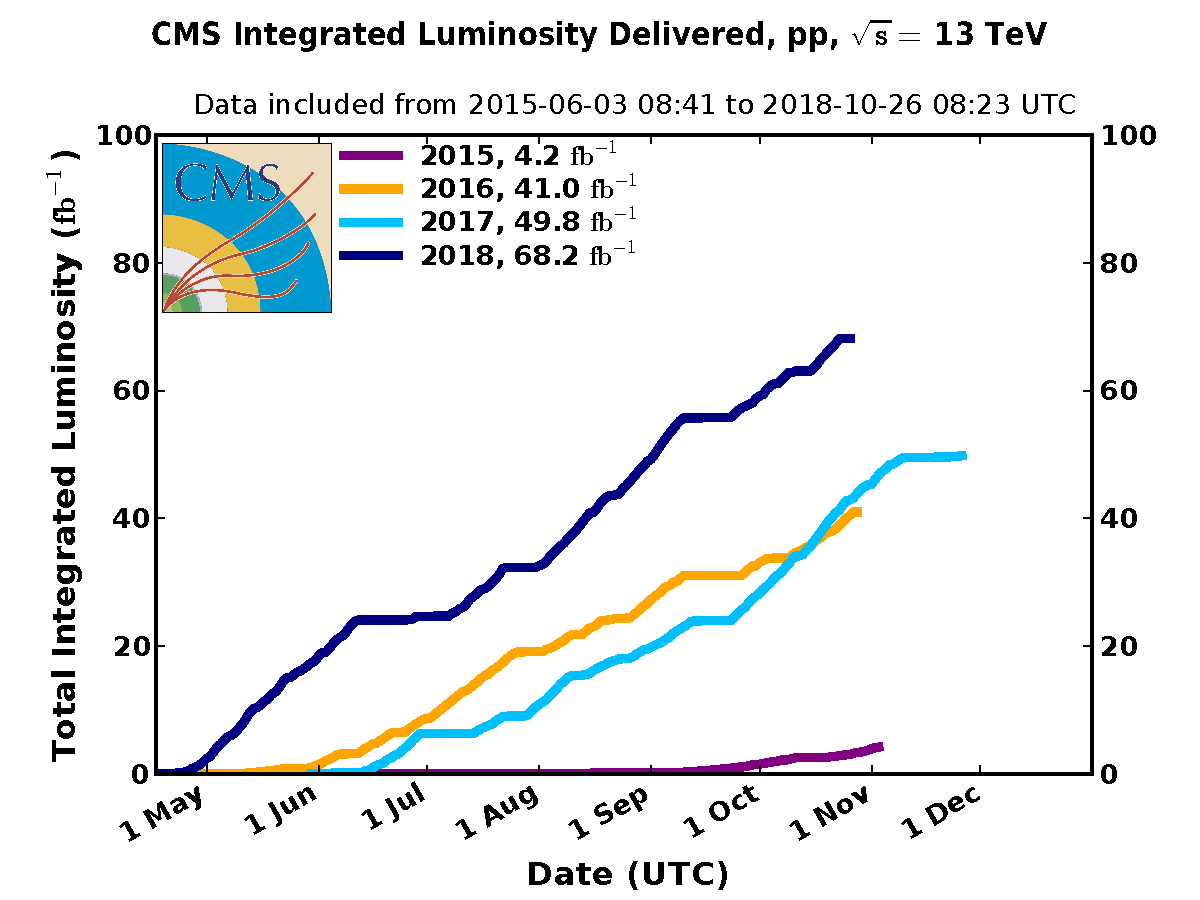
\includegraphics[width=0.5\textwidth]{figures/cms/lumi.pdf}
        \label{fig:cms:lumi}
        \caption{Integrated luminosity of the LHC during proton collisions during the 2016 data-taking period~\cite{lumitwiki}.}
    \end{center}
\end{figure}

\section{The Compact Muon Solenoid}

The Compact Muon Solenoid (CMS)~\cite{cmsjinst} is one of two general purpose LHC detectors (the other being ATLAS).
It is designed to detect and measure stable hadrons, photons, electrons, and muons produced in proton and ion collisions at LHC interaction point 5. 
From these event descriptions, a number of physics processes can be probed, including SM measurements~\needcite, BSM searches~\needcite, and the discovery of the Higgs boson~\needcite. 
In what follows, we will use the $(r,\phi,\eta)$ coordinate system with respect to the $z$ axis:
\begin{itemize}
    \item[$z = $] distance along beam axis, with $z=0$ defined to be at the center of the detector
    \item[$r = $] distance from the $z$ axis
    \item[$\phi = $] azimuthal angle in the plane orthogonal to the $z$ axis
    \item[$\eta = $]$-\log\nicefrac{\theta}{2}$ (pseudorapidity), where $\theta$ is the angle from the $z$ axis
\end{itemize}
In this coordinate system, we define $x$ and $y$ to lie in the plane perpendicular to $z$, with $x$ pointing from the center of the detector to the center of the LHC.
As with the pseudorapidity, it is convenient to use quantities invariant under $z$-boosts, and so we define the transverse momentum:
\begin{equation}
    \vec{p}_\mathrm{T} = \left(\begin{matrix} p_x \\ p_y \end{matrix}\right)
\end{equation}
We will frequently make use of the magnitude of this vector, $\pt$. 
CMS can detect collision products that are within the fiducial volume of $0 \leq \phi < 2\pi$ and $-5 \leq \eta\leq 5$. 
Several detector subsystems are used to identify and reconstruct muons, electrons, photons, and charged and neutral hadrons. 

\subsubsection{Silicon tracker}

Starting from the beam pipe, the first of these subsystems is the silicon tracker~\cite{cmstracker}, used to identify charged particles and measure their momenta. 
The tracker consists of silicon detector geometries: pixels (providing 3D position measurement) and strips (2D). 
The arrangement of the pixel and strip layers are shown in Figure~\ref{fig:cms:si}.
The tracker sits in a near-uniform 3.8 T magnetic field, produced by a superconducting NbTi solenoid. 
The field lines in the tracker volume are approximately parallel to the beam pipe. 

A single silicon pixel has dimensions $285\times100\times150$ $(\mu\mathrm{m})^3$ (in $r\times r\phi\times z$), leading to a position resolution of $\sim10\times30$ $(\mu\mathrm{m})^2$ (in $r\phi\times z$). 
The 66 million pixels are arranged into 7 layers: 3 cylindrical ``barrels'' (at $r=4.4,~7.3,~10.2$ cm) and $2\times2$ ``endcap'' annulli (at $z=\pm34.5,~\pm46.5$ cm). 
Outside the pixel layers are the strip layers, consisting of 9.3 million silicon strips arranged into barrels and endcaps.
The resolution in $r\phi$ varies between $10$ and $50$ $\mu$m, depending on the location and pitch of the given strip.
Certain strip layers contain two layers of strips, rotated through a ``stereo'' angle (100 mrad) with respect to each other.
By matching adjacent hits, the stereo measurement can add a third dimension ($z$ for barrel, $r$ for endcap) to the strip's 2D measurement, with resolution $100$-$500$ $\mu$m.
There are a total of 10 barrel layers ($0.2 < r < 1$ m) and 24 endcap layers ($0.6 < |z| < 2.8$ m). 

\begin{figure}
    \begin{center} 
        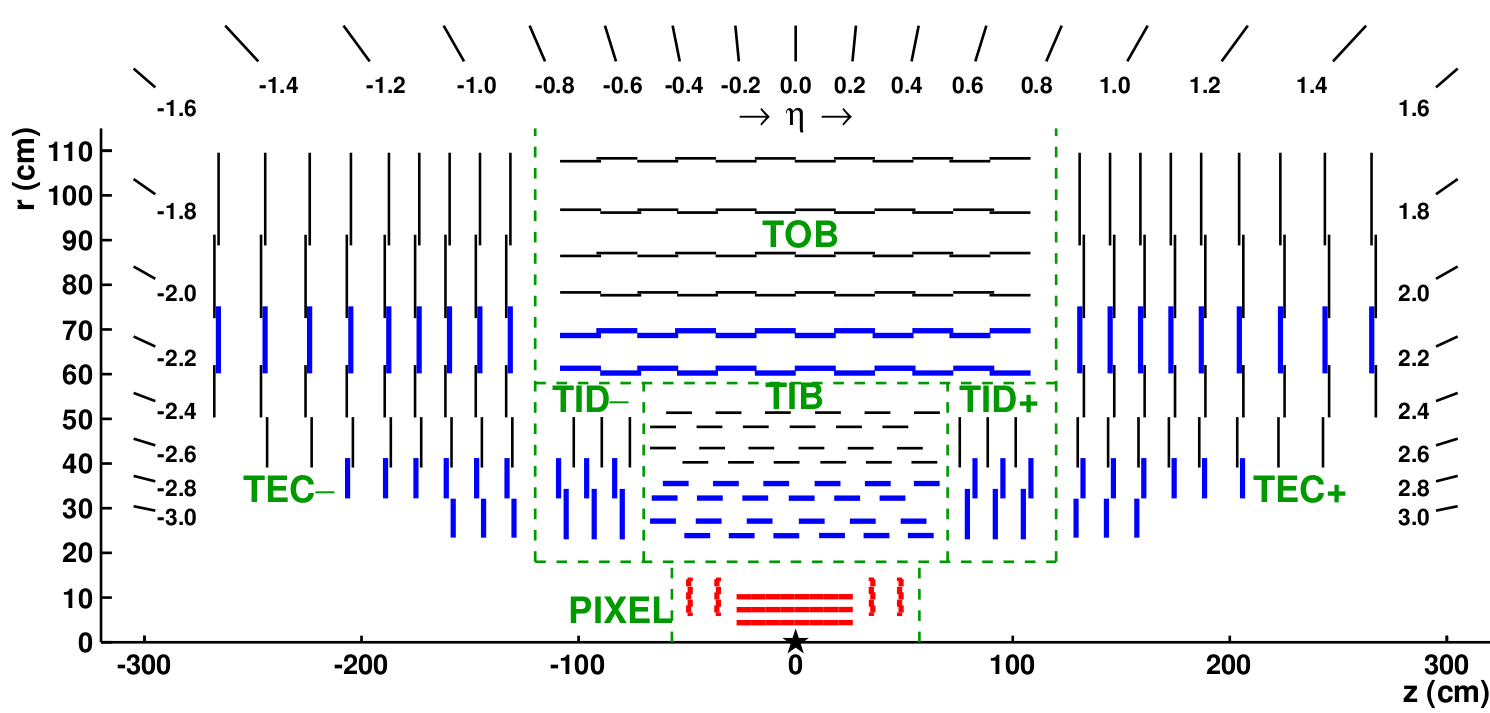
\includegraphics[width=0.7\textwidth]{figures/cms/tracker.png}
        \caption{Diagram of a slice of the CMS tracking system.
                 The pixel layers are shown in bold red lines.
                 Single-strip (double-strip) layers are indicated by thin black (bold blue) lines.
                 The double-strip modules each consist of two back-to-back strips, rotated with respect to each other, that can provide 3D localization of the hits.
                 Adapted from Reference~\cite{cmstracker}.}
        \label{fig:cms:si}
    \end{center}
\end{figure}

Pixels with a signal greater than a tuneable readout threshold (typically around $3000 Q_e$) are read out.
These pixels are then aggregated with adjacent signals to form pixel clusters, which are further subjected to readout thresholds ($\sim 4000 Q_e$).
The exact position of the particle in this layer (known as a ``hit'') is inferred by fitting the charge distribution of the pixels in this cluster to pre-determined templates.
A similar method is employed to determine the strip hit positions, with some modifications to account for Lorentz drift of the charges in the silicon detector due to the $B$-field. 
The efficiency of reconstructing hits varies with the detector type, location, and particle momentum, but is generally greater than $99\%$ ($99.5\%$ if defective modules are not considered). 

Tracks are found using an iterative ``inside-out'' process, where each iteration has five steps:
\begin{enumerate}
    \item Define seeds using pixel hits, double-strip hits (i.e. hits with 3D information), and an estimate of the beam spot (collision point). At least 3 hits are needed for the seed.
    \item Use a Kalman filter~\needcite to evolve track seeds through the rest of the tracker and find hits, accounting for the $B$-field and energy loss.
    \item Estimate trajectory parameters after finding all hits.
    \item Decide whether to keep found tracks based on quality requirements (e.g. number of missing hits)
    \item Remove hits associated with tracks from hit collection and repeat.
\end{enumerate}
The trajectory parameters referred to in step 3 are the 5 parameters of a helix: $\rho$ (curvature), $\phi_0$ (azimuthal angle), $\lambda$ ($\cot\theta$), $d_0$ (``impact parameter'', minimum $r$ of track), $z_0$ (minimum $|z|$ of track).
The CMS track fit typically has 5-6 iterations, with each successive iteration loosening the seed and track fit requirements to look for more difficult tracks (e.g. missing hits, large $d_0$).
The efficiency and fake rate of this process, as a function of track \pt, are shown in Figure~\ref{fig:cms:trackeff}.
For muons with $|\eta|<1.5$ and $\pt>1$ GeV, the tracking efficiency is over 98\%, with a combinatorial fake rate of 2-6\%. 

\begin{figure}
    \begin{center} 
        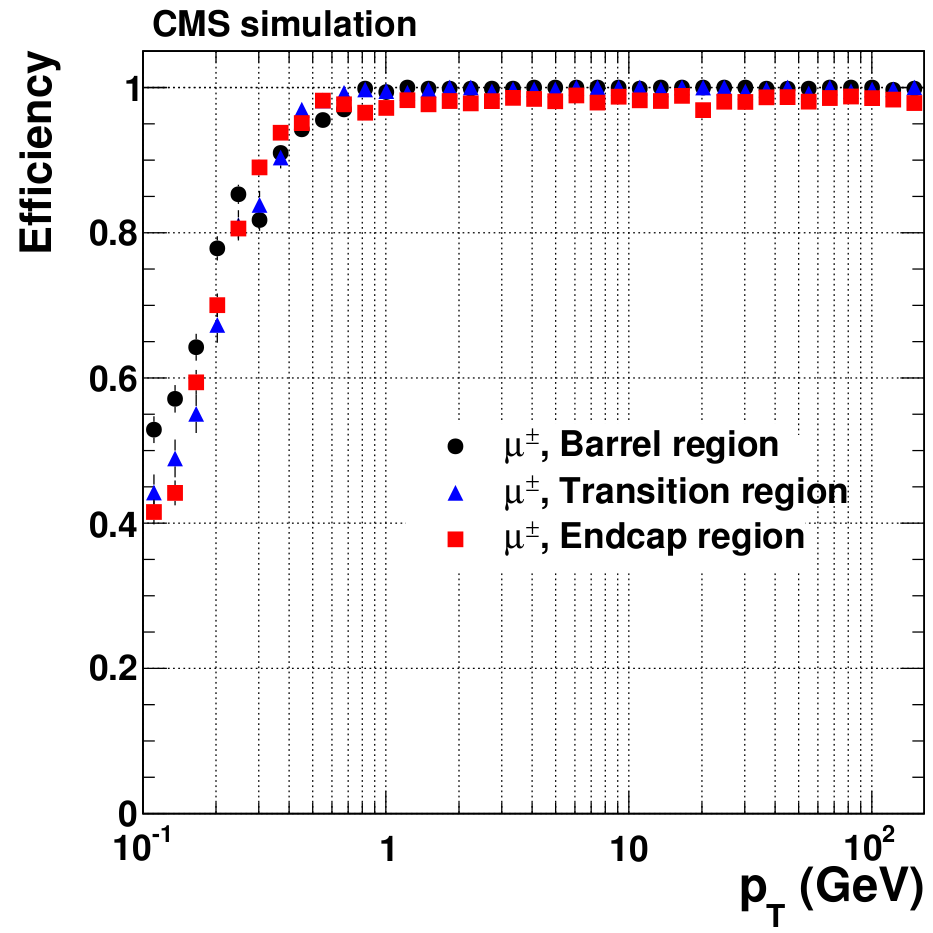
\includegraphics[width=0.35\textwidth]{figures/cms/track_eff.png}
        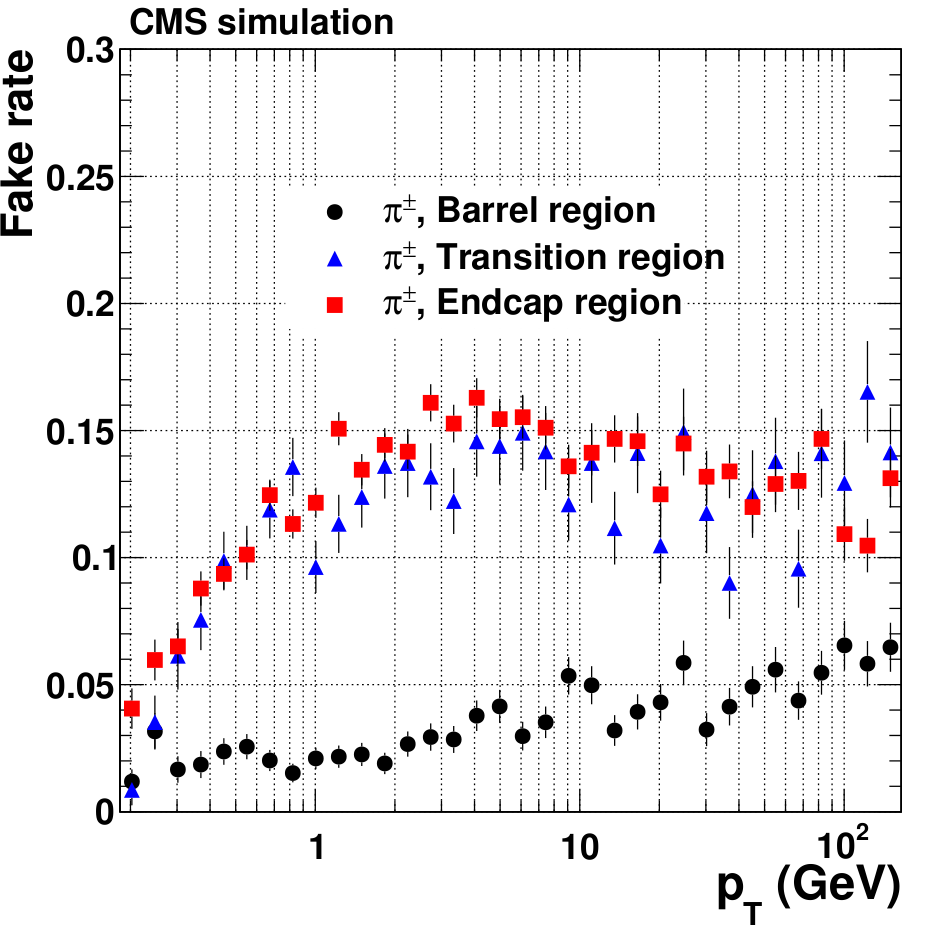
\includegraphics[width=0.35\textwidth]{figures/cms/track_fake.png}
        \caption{Efficiency (fake rate) of the CMS track fit algorithm, evaluated using simulation of muons (charged pions).}
        \label{fig:cms:trackeff}
    \end{center}
\end{figure}


\subsubsection{Electromagnetic calorimetry}

The CMS electromagnetic calorimeter~\cite{cmsecaljinst} (ECAL) is a homogenous detector with good energy and angular resolution, composed of 76,000 \pbwo~crystals. 
The crystals are arranged in two sections: a cylindrical barrel (EB) covering $|\eta|<1.44$ and two endcap annuli (EE) extending to $|\eta|<3$.
This provides slightly more coverage than the tracking volume.
Each crystal in the EB (EE) has dimensions $2.2\times2.2\times23$ ($2.68\times2.68\times22$) $(\mathrm{cm}^3)$, with the long dimension pointing towards the beam.
This can be compared to a Moli\'ere radius $r_M=2.19$ cm and a radiation length of $X_0=0.89$ cm. 
A cross-sectional area comparable to $r_M\times r_M$ facilitates the differentiation of different electromagnetic (EM) showers arising from electrons and photons.
The depth of the crystal (in units of $X_0$) drives the excellent energy resolution, which is determined using a standalone electron beam:
\begin{equation}
    \frac{\sigma_E}{E} = \frac{2.8\%}{\sqrt{E/\mathrm{GeV}}} \oplus \frac{12\%}{E/\mathrm{GeV}} \oplus 0.3\%
\end{equation}
Scintillation photons from the \pbwo~crystals are collected by avalanche photodiodes (APDs) in the EB and vacuum phototriodes (VPTs) in the EE, which provide amplification factors of 50 and 10, respectively. 

At high momenta, the two photons from a $\pi^0$ decay may merge into a single ECAL crystal. 
This primarily occurs at high $|\eta|$ due to the $z$-boost of the intitial state.
To differentiate one- and two-photon deposits, a ``preshower'' detector sits in front of the EE ($1.6 < |\eta|<2.5$).
The preshower detector consists of a lead absorber and silicon strips.
A photon (or photon pair) initiates a shower in the lead.
The shower can be resolved in the silicon strips, which have resolution $\mathcal{O}(1\mathrm{-}10)$ mm.

The physical placement of all three ECAL components is shown in Figure~\ref{fig:cms:ecal}.

\begin{figure}
    \begin{center} 
        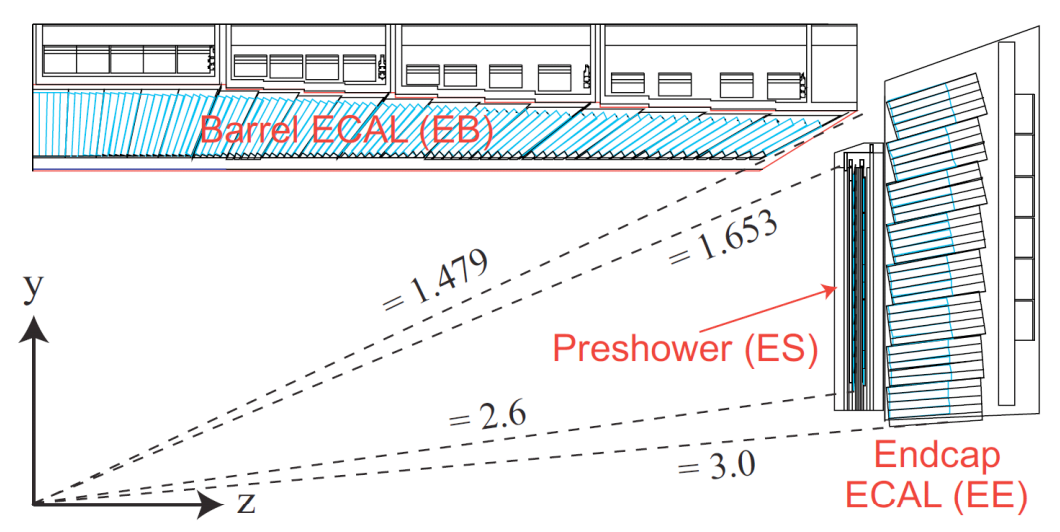
\includegraphics[width=0.7\textwidth]{figures/cms/ecal.png}
        \caption{One quadrant of the CMS ECAL (symmetric with rotation around $z$ and reflection across $z=0$).
                 The dashed lines indicate values of $\eta$.
                 Adapted from Reference~\cite{cmsecaljinst}.}
        \label{fig:cms:ecal}
    \end{center}
\end{figure}


\subsubsection{Hadronic calorimetry}

\subsubsection{Muon chambers}

\subsubsection{Online trigger system}

\section{Simulation of collisions}

\subsection{Physics simulation}

\subsection{Detector simulation}

\section{Particle reconstruction algorithms}

\subsubsection{Tracks and vertices}

\subsubsection{Electrons and photons}

\subsubsection{Jets}

\subsubsection{Muons}

\subsubsection{Particle flow algorithm}

\subsubsection{Missing momentum}

